\documentclass[letterpaper,12pt]{article}

\usepackage{tabularx} % extra features for tabular environment
\usepackage{amsmath}  % improve math presentation
\usepackage{graphicx} % takes care of graphic including machinery
\usepackage[margin=1in,letterpaper]{geometry} % decreases margins
\usepackage[final]{hyperref} % adds hyper links inside the generated pdf file
\usepackage{ctex}
\usepackage{titlesec}
%\usepackage{CJKutf8, CJK}
\usepackage{makecell}                 % 三线表-竖线
\usepackage{booktabs}                 % 三线表-短细横线
% \usepackage{natbib}
\usepackage{graphicx}				  % 表格单元格逆时针
\usepackage{multirow}				  % 合并单元格
\usepackage{array}
\usepackage{amssymb}				  % 勾
\usepackage{amsmath}
\usepackage{longtable}                % 导入 longtable 宏包,表格自动换行
\usepackage{caption}
\usepackage{subcaption}               % 设置子图
\usepackage{color}					  % 文本颜色包
\usepackage{xcolor}
\usepackage{bbm}					  % 输入指示函数
\usepackage{tablefootnote}			  % 表格注释
\usepackage{pythonhighlight}
\usepackage{fancyhdr}
\usepackage{lastpage}
\pagestyle{fancy}
\fancyhf{}
\fancyhead{}
\fancyfoot{}
\fancyhead[R]{\small Page \thepage\ of \pageref*{LastPage}}
\fancyhead[L]{\small Assignment: Self-Attention, Transformers, and Pretraining}
\usepackage{listings}                 % 导入代码块
\usepackage{xcolor}
\lstset{
	numbers=none, 
	tabsize=1,
	columns=flexible, 
	%numberstyle=  \small, 
	%keywordstyle= \color{blue!70},
	commentstyle= \color{green!50!blue!100}, 
	%frame=shadowbox, % 阴影效果
	frame=tlrb
	rulesepcolor= \color{red!20!green!20!blue!20} ,
	%escapeinside=``, % 英文分号中可写入中文
	%xleftmargin=2em,
	%xrightmargin=2em, 
	aboveskip=1em,
} 

\hypersetup{
	colorlinks=true,       % false: boxed links; true: colored links
	linkcolor=blue,        % color of internal links
	citecolor=blue,        % color of links to bibliography
	filecolor=magenta,     % color of file links
	urlcolor=blue       
}

%++++++++++++++++++++++++++++++++++++++++
\titleformat{\section}{\large\bfseries\songti}{\thesection}{1em}{}
\titleformat{\subsection}{\large\bfseries\songti}{\thesubsection}{1em}{}
\titleformat{\subsubsection}{\normalsize\bfseries\songti}{\thesubsubsection}{1em}{}
\titleformat{\paragraph}{\small\bfseries\songti}{\paragraph}{1em}{}
\titleformat{\subparagraph}{\footnotesize\bfseries\songti}{\subparagraph}{1em}{}

\begin{document}
	
	
	\title{\songti \zihao{4}高级人工智能课程汇报}
	\author{信息科学与工程学院 \\ \textrm{Gu Rui} \\ 220220942871}
	\date{\textrm{June 25  2023}}
	\maketitle
	
	\renewcommand{\figurename}{Figure} % 可以重新定义abstract,因为ctex会覆盖thebibliography
	% 	\begin{abstract}
		%		In this experiment we studied a very important physical effect by measuring the
		%		dependence of a quantity $V$ of the quantity $X$ for two different sample
		%		temperatures.  Our experimental measurements confirmed the quadratic dependence
		%		$V = kX^2$ predicted by Someone's first law. The value of the mystery parameter
		%		$k = 15.4\pm 0.5$~s was extracted from the fit. This value is
		%		not consistent with the theoretically predicted $k_{theory}=17.34$~s. We attribute %this
		%		discrepancy to low efficiency of our $V$-detector.
		%	\end{abstract}
	\renewcommand{\contentsname}{Contents}
	\renewcommand{\tablename}{Table}
	\tableofcontents  % 自动生成目录
	
	\section{Attention exploration (22 points)}
	
	\noindent Multi-headed self-attention is the core modeling component of Transformers. In this question, we'll get some practice working with the self-attention equations, and motivate why multi-headed self-attention can be preferable to single-headed self-attention.
	Recall that attention can be viewed as an operation on a \textit{query} $q \in \mathbb{R}^d$, a set of \textit{value} vectors $\{v_1, . . . , v_n \}$, $v_i \in
	\mathbb{R}^d$, and a set of \textit{key} vectors $\{k_1, . . . , k_n\}$, $k_i \in \mathbb{R}^d$, specified as follows:
	
	\begin{equation}
		\begin{aligned}
			c = \sum_{i=1}^{n} v_{i}\alpha_{i}
		\end{aligned}
		\label{eq: Attention_formula_1}
	\end{equation}
	
	\begin{equation}
		\begin{aligned}
			\alpha_{i} = \frac{\exp(k_{i}^{T}q)}{\sum_{j=1}^{n} \exp(k_{j}^{T}q)}
		\end{aligned}
		\label{eq: Attention_formula_2}
	\end{equation}
	with $α_i$ termed the “attention weights”. Observe that the output $c \in \mathbb{R}^d$
	is an average over the value vectors weighted with respect to $α_i$.
	

	\noindent(a) (4 points) \textbf{Copying in attention.} One advantage of attention is that it's particularly easy to “copy” a value vector to the output c. In this problem, we'll motivate why this is the case.
		
	\begin{itemize}
	\item [i.]
	(1 point) \textbf{Explain} why $\alpha$ can be interpreted as a categorical probability distribution.
			
	\textcolor{red}{\textbf{Answer:} Eq.\ref{eq: Attention_formula_1} has shown that this is a fuzzy query, and we cannot directly match a key vector k with the query vector $q$, and can only give each key a certain probability distribution weight (i.e. $\alpha_{ij}$) to get the final output result.}

	\item [ii.]
	(2 points) The distribution $\alpha$ is typically relatively “diffuse”; the probability mass is spread out between many different $\alpha_i$. However, this is not always the case. \textbf{Describe} (in one sentence) under what conditions the categorical distribution $\alpha$ puts almost all of its weight on some $\alpha_j$ , where $j \in \{1, \ldots , n\} (i.e. \quad \alpha_j \gg \sum_{i\neq j} \alpha_i)$. What must be true about the query $q$ and/or the keys $\{k_1, \ldots , k_n\}$?
			
	\textcolor{red}{\textbf{Answer:} According to the calculation method of Eq.\ref{eq: Attention_formula_2}, if the query vector $q$ has a very high similarity to a key $k_i$ (the dot product is large), and $q$ is basically vertical to other bonds (the point product is zero), then $\alpha_i$ will be maximized.}

	\item [iii.]
	(1 point) Under the conditions you gave in (ii), \textbf{describe} what properties the output c might have.
			
	\textcolor{red}{\textbf{Answer:} Under the conditions described in (ii), the output vector $c$ will be heavily influenced by the value vector $v_j$ associated with the key vector $k_j$ that received the majority of the attention weight. At this point, the $c$ is approximately equal to $v_i$}

    \item [iv.]
	(1 point) \textbf{Explain} (in two sentences or fewer) what your answer to (ii) and (iii) means intuitively.
			
	\textcolor{red}{\textbf{Answer:} When the dot product (similarity) between a specific word key and a query significantly outweighs the dot products of other word keys with the same query, the attention output corresponding to that specific word will closely resemble its associated value. This behavior can be likened to "copying" the value into the output.}
	\end{itemize}	
		
	\noindent(b) (7 points) \textbf{An average of two}. Instead of focusing on just one vector $v_j$ , a Transformer model might want to incorporate information from \textit{multiple} source vectors. Consider the case where we instead want to incorporate information from \textbf{two} vectors $v_a$ and $v_b$, with corresponding key vectors $k_a$ and $k_b$.
	
	\begin{itemize}
	\item [i.]
	(3 points) How should we combine two d-dimensional vectors $v_a$, $v_b$ into one output vector $c$ in a way that preserves information from both vectors? In machine learning, one common way to do so is to take the average:  $c = \frac{1}{2}(v_a + v_b)$. It might seem hard to extract information about the original vectors va and $v_b$ from the resulting $c$, but under certain conditions one can do so.
	In this problem, we'll see why this is the case.
			
	\vspace{1em}
			
	Suppose that although we don't know $v_a$ or $v_b$, we do know that $v_a$ lies in a subspace $A$ formed by the $m$ basis vectors $\{a_1, a_2, \ldots , a_m\}$, while $v_b$ lies in a subspace $B$ formed by the $p$ basis vectors $\{b_1, b_2, \ldots , b_p\}$. (This means that any va can be expressed as a linear combination of its basis vectors, as can $v_b$. All basis vectors have norm 1 and orthogonal to each other.)
			
	Additionally, suppose that the two subspaces are orthogonal; i.e. $a^\top_j b_k = 0$ for all $j$, $k$.
	Using the basis vectors $\{a_1, a_2, \ldots , a_m\}$, construct a matrix $M$ such that for arbitrary vectors $v_a \in A$ and $v_b \in B$, we can use $M$ to extract $v_a$ from the sum vector $s = v_a + v_b$. In other words, we want to construct $M$ such that for any $v_a$, $v_b$, $M_s = v_a$.
			
	\textbf{Note:} both $M$ and $v_a$, $v_b$ should be expressed as a vector in $\mathbb{R}^d$, not in terms of vectors from $A$ and $B$.
			
	\textbf{Hint:} Given that the vectors $\{a_1, a_2, \ldots , a_m\}$ are both \textit{orthogonal} and \textit{form a basis} for $v_a$, we know that there exist some $c_1, c_2, \ldots , c_m$ such that $v_a = c_1a_1 + c_2a_2 + \ldots + c_ma_m$. Can you create a vector of these weights $c$?
			
	\textcolor{red}{\textbf{Answer:} Assume that $A$ is a matrix of concatenated basis vectors $\{\mathbf{a}_1, \mathbf{a}_2,\ldots, \mathbf{a}_m\}$ and $B$ is a matrix of concatenated basis vector $\{\mathbf{b}_1, \mathbf{b}_2,\ldots, \mathbf{b}_p\}$.  Linear combinations of vectors $v_a$ and $v_b$ can then be expressed as:
	\begin{equation*}
		\begin{aligned}
			\mathbf{v}_a=c_1\mathbf{a}_1+c_2\mathbf{a}_2+ \ldots + c_m\mathbf{a}_m = \sum_{i=1}^{m} c_i\mathbf{a}_i = A\mathbf{c}
		\end{aligned}
		\label{eq: ai_vector-weighted_sum}
	\end{equation*}
	\begin{equation*}
		\begin{aligned}
			\mathbf{v}_b=d_1\mathbf{b}_1+d_2\mathbf{b}_2+ \ldots + d_p\mathbf{b}_m = \sum_{j=1}^{p} d_j\mathbf{b}_j = B\mathbf{d}
		\end{aligned}
		\label{eq: bj_vector-weighted_sum}
	\end{equation*}
	We need to construct such $M$ which, when multiplied with $\mathbf{v}_b$, produces $\mathbf{0}$ and, when multiplied with $\mathbf{v}_a$, produces the same vector (in terms of its own space). Let $M$ have the following form:
	\begin{equation*}
		\begin{aligned}
			M = \sum_{i=1}^{m}\lambda_i \mathbf{a}_i\mathbf{a}_i^\top
		\end{aligned}
		\label{eq: M_assumed}
	\end{equation*}
	Where $\lambda_i, i=1,\ldots, m$ is the undetermined coefficient, it is derived as follows
	\begin{equation*}
		\begin{aligned}
			M\mathbf{s}=\mathbf{v}_a &\Leftrightarrow M\mathbf{v}_a + M\mathbf{v}_b=\mathbf{v}_a \\
			&\Leftrightarrow \left(\sum_{i=1}^{m}\lambda_i \mathbf{a}_i \mathbf{a}_i^\top \right)\left(\sum_{i=1}^{m} c_i \mathbf{a}_i + \sum_{j=1}^{p} d_i \mathbf{b}_i \right) = \sum_{i=1}^{m} c_i \mathbf{a}_i \\
			&\Leftrightarrow \sum_{i=1}^{m} \lambda_i c_i \mathbf{a}_i \mathbf{a}_i^\top \mathbf{a}_i = \sum_{i=1}^{m} c_i \mathbf{a}_i  \quad \text{(orthogonal property)} \\	
			&\Leftrightarrow \sum_{i=1}^{m} (\lambda_i c_i \mathbf{a}_i^\top \mathbf{a}_i) \mathbf{a}_i = \sum_{i=1}^{m} c_i \mathbf{a}_i \\
			&\Rightarrow \lambda_i c_i \mathbf{a}_i^\top \mathbf{a}_i = c_i \\
			&\Rightarrow \lambda_i = \frac{1}{\mathbf{a}_i^\top \mathbf{a}_i}, i=1,\ldots, m.
		\end{aligned}
		\label{eq: M_solution}
	\end{equation*}
	It is easy to see that, since $\mathbf{a}_j^\top b_k = 0$ for all $j, k$, $A^\top B = 0$. And we know that in terms of $\mathbb{R}^d$ (not in terms of $A$ and $B$), $\mathbf{v}_a$ is just a collection of constants $c$. Thus the results of M are as follows
	\begin{equation*}
		\begin{aligned}
			M = \sum_{i=1}^{m}\frac{\mathbf{a}_i \mathbf{a}_i^\top}{\mathbf{a}_i^\top \mathbf{a}_i} = A^\top
		\end{aligned}
	\label{eq: M_result}
 	\end{equation*}
	} 
			
			
	\item[ii.]
	(4 points) As before, let $v_a$ and $v_b$ be two value vectors corresponding to key vectors $k_a$ and $k_b$, respectively. Assume that (1) all key vectors are orthogonal, so $k_i^\top k_j$ for all $i \neq j$; and (2) all key vectors have norm 1.\footnote{Recall that a vector x has norm 1 if $x^{\top}x = 1$.} \textbf{Find an expression} for a query vector $q$ such that $c \approx \frac{1}{2}(v_a +v_b)$.\footnote{Hint: while the softmax function will never exactly average the two vectors, you can get close by using a large scalar multiple in the expression.}
	
	\textcolor{blue}{\textbf{Thoughts:} In essence is to find a $q$ makes $\mathbf{k}_a^\top q = \mathbf{k}_b^\top q$, then we know $q^\top (\mathbf{k}_a - \mathbf{k}_b) = 0$, to find a $q$ perpendicular to $\mathbf{k}_a - \mathbf{k}_b$}.
	
	\textcolor{red}{\textbf{Answer:} Assume that $c$ is approximated as follows:
	\begin{equation*}
		\begin{aligned}
			c \approx \frac{1}{2}\mathbf{v}_a + \frac{1}{2}\mathbf{v}_b
		\end{aligned}
	\end{equation*}
	This means we want $\alpha_a \approx 0.5$ and $\alpha_b \approx 0.5$, which can be achieved when (whenever $i \neq a$ and $i \neq b$):
	\begin{equation*}
		\begin{aligned}
			\mathbf{k}_a^\top q \approx \mathbf{k}_b^\top q \gg \mathbf{k}_i^\top \mathbf{q}
		\end{aligned}
	\end{equation*}
	Like explained in the previous question, if the dot product is big, the probability mass will also be big and we want a balanced mass between $\alpha_a$ and $\alpha_b$. $q$ will be largest for $k_a$ and $k_b$ when it is a large multiplicative of a vector that contains a component in $k_a$ direction and in $k_b$ direction:
	\begin{equation*}
		\begin{aligned}
			\mathbf{q} = \beta (\mathbf{k}_a + \mathbf{k}_b), \quad \text{where} \beta \gg 0
		\end{aligned}
	\end{equation*}
	Now, since the keys are orthogonal to each other, it is easy to see that:
	\begin{equation*}
		\begin{aligned}
			\mathbf{k}_a^\top q = \beta; \mathbf{k}_b^\top q = \beta; \mathbf{k}_i^\top q = 0, \quad \text{whever} \ i\neq a \ \text{and} \ i\neq b
		\end{aligned}
	\end{equation*}
	Thus when we exponentiate, only $\exp(\beta)$ will matter, because $\exp(0)$ will be insignificant to the probability mass. We get that:
	\begin{equation*}
		\begin{aligned}
			\alpha_a=\alpha_b=\frac{\exp(\beta)}{n-2+2\exp(\beta)} \approx \frac{\exp(\beta)}{2\exp(\beta)} \approx \frac{1}{2}, \ \text{for} \ \beta \gg 0
		\end{aligned}
	\end{equation*}
	}
	
	\end{itemize}	
	
	
	
	\noindent(c) (5 points) \textbf{Drawbacks of single-headed attention:} In the previous part, we saw how it was \textit{possible} for a single-headed attention to focus equally on two values. The same concept could easily be extended to any subset of values. In this question we'll see why it's not a practical solution. Consider a set of key vectors $\{k_1, \ldots , k_n\}$ that are now randomly sampled, $k_i \sim \mathcal{N}(μ_i,\Sigma_i)$, where the means $μ_i \in \mathbb{R}^d$ are known to you, but the covariances $\Sigma_i$ are unknown. Further, assume that the means $μ_i$ are all perpendicular; $\mu^\top_i \mu_j = 0$ if $i \neq j$, and unit norm, $\|\mu_i\| = 1$.
	
	\begin{itemize}
	\item[i.]
	(2 points) Assume that the covariance matrices are $\Sigma_i = \alpha I \forall i \in {1, 2, \ldots , n}$, for vanishingly small $\alpha$. Design a query $q$ in terms of the $\mu_i$ such that as before, $c \approx \frac{1}{2}(v_a +v_b)$, and provide a brief argument as to why it works.
		
	\item[ii.]
	(3 points) Though single-headed attention is resistant to small perturbations in the keys, some types of larger perturbations may pose a bigger issue. Specifically, in some cases, one key vector $k_a$ may be larger or smaller in norm than the others, while still pointing in the same direction as $\mu_a$. As an example, let us consider a covariance for item $a$ as $\Sigma_a = \alpha I+ \frac{1}{2}(\mu_a\mu^\top_a )$ for vanishingly small $\alpha$ (as shown in Fig. \ref{fig: vector}). This causes $k_a$ to point in roughly the same direction as $\mu_a$, but with large variances in magnitude. Further, let $\Sigma_i = \alpha I$ for all $i \neq a$.
		
	\begin{figure}[htbp] 
		% read manual to see what [ht] means and for other possible options
		\centering 
		% \includegraphics[width=0.8\columnwidth]{GLADNet}
		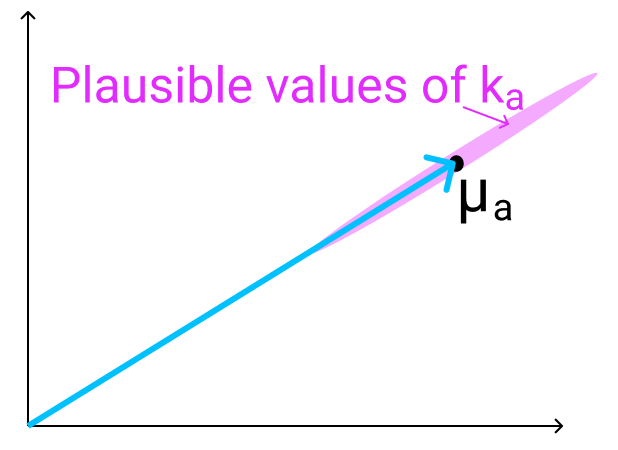
\includegraphics[width=0.5\linewidth]{ka_plausible}
		\captionsetup{font=small}
		\label{vector}
		\caption{
			\label{fig: vector} % spaces are big no-no withing labels
			% things like fig: are optional in the label but it helps
			% to orient yourself when you have multiple figures,
			% equations and tables
			The vector $\mu_a$ (shown here in 2D as an example), with the range of possible values of $k_a$ shown in red. As mentioned previously, $k_a$ points in roughly the same direction as $\mu_a$, but may have larger or smaller magnitude.
		}
	\end{figure}
		
	When you sample $\{k_1, \ldots , k_n\}$ multiple times, and use the $q$ vector that you defined in part i., what qualitatively do you expect the vector $c$ will look like for different samples?

	\end{itemize}	
	
	\noindent (d) (3 points) \textit{Benefits of multi-headed attention:} Now we'll see some of the power of multi-headed attention. We'll consider a simple version of multi-headed attention which is identical to single-headed self-attention as we've presented it in this homework, except two query vectors ($q_1$ and $q_2$) are defined, which leads to a pair of vectors ($c_1$ and $c_2$), each the output of single-headed attention given its respective query vector. The final output of the multi-headed attention is their average,$\frac{1}{2}(c_1+c_2)$. As in question 1(c), consider a set of key vectors $\{k_1, \ldots , k_n\}$ that are randomly sampled, $k_i \sim \mathcal{N} (\mu_i, \Sigma_i)$, where the means $\mu_i$ are known to you, but the covariances $\Sigma_i$ are unknown. Also as before,	assume that the means µi are mutually orthogonal; $\mu^\top_i \mu_j = 0$ if $i \neq j$, and unit norm,$\|\mu_i\|= 1$.
	
	\begin{itemize}
	\item[i.] 
	(1 point) Assume that the covariance matrices are $\Sigma_i = \alpha I$, for vanishingly small $\alpha$. Design $q_1$
	and $q_2$ such that $c$ is approximately equal to $\frac{1}{2}(v_a + v_b)$.
	
	\item[ii.] 
	(2 points) Assume that the covariance matrices are $\Sigma_a = \alpha I + \frac{1}{2}(\mu_a \mu_a^\top)$ for vanishingly small $\alpha$, and $\Sigma_i = \alpha I$ for all $i \neq a$. Take the query vectors $q_1$ and $q_2$ that you designed in part i.
	
	What, qualitatively, do you expect the output $c$ to look like across different samples of the key
	vectors? Please briefly explain why. You can ignore cases in which $k^\top_a q_i < 0$.
	\end{itemize}	
	
	\section{Pretrained Transformer models and knowledge access (35 points)}
	
	\noindent You'll train a Transformer to perform a task that involves accessing knowledge about the world – knowledge which isn't provided via the task's training data (at least if you want to generalize outside the training set). You'll find that it more or less fails entirely at the task. You'll then learn how to pretrain that Transformer on Wikipedia text that contains world knowledge, and find that finetuning that Transformer on the same knowledge-intensive task enables the model to access some of the knowledge learned at pretraining time. You'll find that this enables models to perform considerably above chance on a held out development set.
	
	\noindent The code you're provided with is a fork of Andrej Karpathy's \textcolor{blue}{minGPT\footnote{https://github.com/karpathy/minGPT}}. It's nicer than most research code in that it's relatively simple and transparent. The “GPT” in minGPT refers to the Transformer language model of OpenAI, originally described in \textcolor{blue}{this paper} \cite{b1}.
	
	\noindent As in previous assignments, you will want to develop on your machine locally, then run training on HuaWei Could. Youll need around 5 hours for training, so budget your time accordingly!

	\noindent Your work with this codebase is as follows:
	
	\begin{itemize}
	\item[(a)]
		(0 points)\textbf{Check out the demo.}\\
		In  the mingpt-demo/ folder is a Jupyter notebook that trains and samples from a Transformer language model. Take a look at it (locally on your computer) to get somewhat familiar with how it defines and trains models. Some of the code you're writing below will be inspired by what you see in this notebook.
		
		Note that you do not have to write any code or submit written answers for this part.
		
	\item[(b)]
		(0 points)\textbf{Read through \texttt{NameDataset}, our dataset for reading name-birthplace pairs.}\\
		The task we'll be working on with our pretrained models is attempting to access the birth place of a notable person, as written in their Wikipedia page.
		We'll think of this as a particularly simple form of question answering:
		\begin{quote}
			\textit{Q: Where was \textit{[person]} born?}\\
			\textit{A: [place]}
		\end{quote}
		From now on, you'll be working with the \texttt{src/} folder. \textbf{The code in \texttt{mingpt-demo/} won't be changed or evaluated for this assignment.}
		In \texttt{dataset.py}, 
		you'll find the the class \texttt{NameDataset}, which reads a TSV (tab-separated values) file of name/place pairs and produces examples of the above form that we can feed to our Transformer model.
		
		To get a sense of the examples we'll be working with, if you run the following code, it'll load your \texttt{NameDataset} on the training set \texttt{birth\_places\_train.tsv} and print out a few examples.
		\begin{lstlisting}[language=bash]
			python src/dataset.py namedata 
		\end{lstlisting}
		Note that you do not have to write any code or submit written answers for this part.
	
	\item[(c)]
		(0 points)\textbf{Implement finetuning (without pretraining).}\\
		Take a look at \texttt{run.py}. It has some skeleton code specifying flags you'll eventually need to handle as command line arguments.
		In particular, you might want to \textit{pretrain}, \textit{finetune}, or \textit{evaluate} a model with this code. For now, we'll focus on the finetuning function, in the case without pretraining.
		
		Taking inspiration from the training code in the \texttt{play\_char.ipynb} file, write code to finetune a Transformer model on the name/birthplace dataset, via examples from the \texttt{NameDataset} class. For now, implement the case without pretraining (i.e. create a model from scratch and train it on the birthplace prediction task from part (b)). You'll have to modify two sections, marked \texttt{[part c]} in the code: one to initialize the model, and one to finetune it. Note that you only need to initialize the model in the case labeled ``vanilla'' for now (later in section (g), we will explore a model variant).
		Use the hyperparameters for the \texttt{Trainer} specified in the \texttt{run.py} code.
		
		Also take a look at the \textit{evaluation} code which has been implemented for you. It samples predictions from the trained model and calls \texttt{evaluate\_places()} to get the total percentage of correct place predictions. You will run this code in part (d) to evaluate your trained models.
		
		This is an intermediate step for later portions, including Part d, which contains commands you can run to check your implementation. No written answer is required for this part.
		
	\item[(d)]
		(5 points)\textbf{Make predictions (without pretraining).}\\ 
		Train your model on \texttt{birth\_places\_train.tsv}, and evaluate on \texttt{birth\_dev.tsv}. Specifically, you should now be able to run the following three commands:
		\begin{lstlisting}[language=bash, basicstyle=\small\ttfamily]
			# Train on the names dataset
			python src/run.py finetune vanilla wiki.txt \
			--writing_params_path vanilla.model.params \
			--finetune_corpus_path birth_places_train.tsv
			
			# Evaluate on the dev set, writing out predictions
			python src/run.py evaluate vanilla wiki.txt  \
			--reading_params_path vanilla.model.params \
			--eval_corpus_path birth_dev.tsv \
			--outputs_path vanilla.nopretrain.dev.predictions
			
			# Evaluate on the test set, writing out predictions
			python src/run.py evaluate vanilla wiki.txt  \
			--reading_params_path vanilla.model.params \
			--eval_corpus_path birth_test_inputs.tsv \
			--outputs_path vanilla.nopretrain.test.predictions
		\end{lstlisting}
		
		Training will take less than 10 minutes (on Huawei Cloud).  Report your model's accuracy on the dev set (as printed by the second command above). Don't be surprised if it is well below 10\%; we will be digging into why in Part 3. As a reference point, we want to also calculate the accuracy the model would have achieved if it had just predicted ``London'' as the birth place for everyone in the dev set. Fill in \texttt{london\_baseline.py} to calculate the accuracy of that approach and report your result in your write-up. You should be able to leverage existing code such that the file is only a few lines long. 
		
	\item[(e)]
		(10 points)\textbf{Define a \textit{span corruption} function for pretraining.}\\
		In the file \texttt{src/dataset.py}, implement the \texttt{\_\_getitem\_\_()} function for the dataset class \\ \texttt{CharCorruptionDataset}.
		Follow the instructions provided in the comments in \texttt{dataset.py}.
		Span corruption is explored in the \href{https://arxiv.org/pdf/1910.10683.pdf}{T5 paper} \cite{b2}.
		It randomly selects spans of text in a document and replaces them with unique tokens (noising).
		Models take this noised text, and are required to output a pattern of each unique sentinel followed by the tokens that were replaced by that sentinel in the input.
		In this question, you'll implement a simplification that only masks out a single sequence of characters.
		
		This question will be graded via autograder based on whether your span corruption function implements some basic properties of our spec.
		We'll instantiate the \texttt{CharCorruptionDataset} with our own data, and draw examples from it.
		
		To help you debug, if you run the following code, it'll sample a few examples from your \\ \texttt{CharCorruptionDataset} on the pretraining dataset \texttt{wiki.txt} and print them out for you.
		\begin{lstlisting}[language=bash]
			python src/dataset.py charcorruption
		\end{lstlisting}
		
		No written answer is required for this part.
		
	\item[(f)]
		(10 points)\textbf{Pretrain, finetune, and make predictions. Budget 2 hours for training.}\\
		Now fill in the \textit{pretrain} portion of \texttt{run.py}, which will pretrain a model on the span corruption task. Additionally, modify your \textit{finetune} portion to handle finetuning in the case \textit{with} pretraining. In particular, if a path to a pretrained model is provided in the bash command, load this model before finetuning it on the birthplace prediction task.
		Pretrain your model on \texttt{wiki.txt} (which should take approximately two hours), finetune it on \texttt{NameDataset} and evaluate it. Specifically, you should be able to run the following four commands:
		(Don't be concerned if the loss appears to plateau in the middle of pretraining; it will eventually go back down.)
		\begin{lstlisting}[language=bash]
			# Pretrain the model
			python src/run.py pretrain vanilla wiki.txt \
			--writing_params_path vanilla.pretrain.params
			
			# Finetune the model
			python src/run.py finetune vanilla wiki.txt \
			--reading_params_path vanilla.pretrain.params \
			--writing_params_path vanilla.finetune.params \
			--finetune_corpus_path birth_places_train.tsv
			
			# Evaluate on the dev set; write to disk
			python src/run.py evaluate vanilla wiki.txt  \
			--reading_params_path vanilla.finetune.params \
			--eval_corpus_path birth_dev.tsv \
			--outputs_path vanilla.pretrain.dev.predictions
			
			# Evaluate on the test set; write to disk
			python src/run.py evaluate vanilla wiki.txt  \
			--reading_params_path vanilla.finetune.params \
			--eval_corpus_path birth_test_inputs.tsv \
			--outputs_path vanilla.pretrain.test.predictions
		\end{lstlisting}
		
		Report the accuracy on the dev set (printed by the third command above). We expect the dev accuracy will be at least 10\%, and will expect a similar accuracy on the held out test set.
		
	\item[(g)]
		(10 points)\textbf{Research! Write and try out a more efficient variant of Attention (Budget 2 hours for pretraining!)}\\
		
		We'll now go to changing the Transformer architecture itself -- specifically the first and last transformer blocks.
		While we've been using a self-attention scoring function based on dot products, this involves a rather intensive computation that's quadratic in the sequence length. This is because the dot product between $\ell^2$ pairs of word vectors is computed in each computation. \textit{Synthesized attention} \cite{b3} is a very recent alternative that has potential benefits by removing this dot product (and quadratic computation) entirely. It's a promising idea, and one way for us to ask, "What's important/right about the Transformer architecture, and where can we improve/prune aspects of it?" In \texttt{attention.py}, implement the forward() method of SynthesizerAttention, which implements a variant of the Synthesizer proposed in the cited paper.
		
		The provided \texttt{CausalSelfAttention} layer implements the following attention for each head of the multi-headed attention: Let $X\in \mathbb{R}^{\ell \times d}$ (where $\ell$ is the block size and $d$ is the total dimensionality, $d/h$ is the dimensionality per head.).\footnote{Note that these dimensionalities do not include the minibatch dimension.}
		
		Let $Q_i,K_i,V_i \in \mathbb{R}^{d\times d/h}$.
		Then the output of the self-attention head is 
		\begin{equation} \label{qkv_eqn}
			Y_i = \text{softmax}\bigg(\frac{(XQ_i)(XK_i)^\top}{\sqrt{d/h}}\bigg)(XV_i)
		\end{equation}
		where $Y_i\in\mathbb{R}^{\ell \times d/h}$.
		Then the output of the self-attention is a linear transformation of the concatenation of the heads:
		\begin{equation}
			Y = [Y_1;\dots;Y_h]A
		\end{equation}
		where $A \in\mathbb{R}^{d\times d}$ and $[Y_1;\dots;Y_h]\in\mathbb{R}^{\ell \times d}$.
		The code also includes dropout layers which we haven't written here.
		We suggest looking at the provided code and noting how this equation is implemented in PyTorch.

		Your job is to implement the following variant of attention. Instead of Eq. \ref{qkv_eqn}, implement the
		following in SynthesizerAttention:
		\begin{equation}
			Y_i = \text{softmax}\left( \text{ReLU}(XA_i + b_1)B_i + b_2 \right)\left(XV_i\right),
		\end{equation}
		where $A_i \in \mathbf{R}^{d\times d/h}$, $B_i \in \mathbf{R}^{d/h \times \ell}$, and $V_i \in \mathbf{R}^{d \times d/h}$.\footnote{Hint: copy over the CausalSelfAttention class, and modify it minimally for this.} One way to interpret this is as follows: The term $(XQ_i)(XK_i)^\top$ is an $\ell \times \ell$ matrix of attention scores, computed as all pairs of dot products between word embeddings. The synthesizer variant eschews the all-pairs dot product and directly computes the $\ell \times \ell$ matrix of attention scores by mapping each d-dimensional vector of each head for $X$ to an $\ell$-dimesional vector of unnormalized attention weights.
		
		In the rest of the code in the src/ folder, modify your model to support using either CausalSelfAttention or SynthesizerAttention. Add the ability to switch between these attention variants depending on whether "vanilla" (for causal self-attention) or "synthesizer" (for the synthesizer variant) is selected in the command line arguments (see the section marked [part g] in src/run.py). You are free to implement this functionality in any way you choose, so long as it supports these command line arguments.
		
		Below are bash commands that your code should support in order to pretrain the model, finetune it, and make predictions on the dev and test sets.
		Note that the pretraining process will take approximately 2 hours. 
		\clearpage
		\begin{lstlisting}[basicstyle=\ttfamily, language=bash]
			
			# Pretrain the model
			python src/run.py pretrain synthesizer wiki.txt \
					--writing_params_path synthesizer.pretrain.params
			
			# Finetune the model
			python src/run.py finetune synthesizer wiki.txt \
					--reading_params_path synthesizer.pretrain.params \
					--writing_params_path synthesizer.finetune.params \
					--finetune_corpus_path birth_places_train.tsv
			
			# Evaluate on the dev set; write to disk
			python src/run.py evaluate synthesizer wiki.txt \
					--reading_params_path synthesizer.finetune.params \
					--eval_corpus_path birth_dev.tsv \
					--outputs_path synthesizer.pretrain.dev.predictions
			
			# Evaluate on the test set; write to disk
			python src/run.py evaluate synthesizer wiki.txt \
					--reading_params_path synthesizer.finetune.params \
					--eval_corpus_path birth_test_inputs.tsv \
					--outputs_path synthesizer.pretrain.test. predictions
		\end{lstlisting}
		
		Report the accuracy of your perceiver attention model on birthplace prediction on \texttt{birth\_dev.tsv} after pretraining and fine-tuning.
		\begin{itemize}
		\item[i.]
			(8 points)We'll score your model as to whether it gets at least 5\% accuracy on the test set, which has answers held out.
			
		\item[ii.]
			(2 points)Why might the synthesizer self-attention not be able to do, in a single layer, what the key-query-value self-attention can do?
		\end{itemize}
		
	\end{itemize}
	
	
	\section{Considerations in pretrained knowledge (5 points)}
	
	\begin{itemize}
		\item[(a)]
			(1 point) Succinctly explain why the pretrained (vanilla) model was able to achieve an accuracy of above 10\%, whereas the non-pretrained model was not.
		\item[(b)]
			(2 points) Take a look at some of the correct predictions of the pretrain+finetuned vanilla model, as well as some of the errors. We think you'll find that it's impossible to tell, just looking at the output, whether the model retrieved the correct birth place, or made up an incorrect birth place. Consider the implications of this for user-facing systems that involve pretrained NLP components. Come up with two distinct reasons why this model behavior (i.e. unable to tell whether it's retrieved or made up) may cause concern for such applications, and an example for each reason.
		\item[(c)] 
			(2 points) If your model didn't see a person's name at pretraining time, and that person was not seen at fine-tuning time either, it is not possible for it to have “learned” where they lived. Yet, your model will produce something as a predicted birth place for that person's name if asked. Concisely describe a strategy your model might take for predicting a birth place for that person's name, and one reason why this should cause concern for the use of such applications. (You do not need to submit the same answer for 3c as for 3b.)
	\end{itemize}
	
	%	\section{Analysis}
	
	%	In this section you will need to show your experimental results. Use tables and
	%	graphs when it is possible. Table~\ref{tbl:bins} is an example.
	
	%	\begin{table}[ht]
		%		\begin{center}
			%			\caption{Every table needs a caption.}
			%			\label{tbl:bins} % spaces are big no-no withing labels
			%			\begin{tabular}{|ccc|} 
				%				\hline
				%				\multicolumn{1}{|c}{$x$ (m)} & \multicolumn{1}{c|}{$V$ (V)} & \multicolumn{1}{c|}{$V$ (V)} \\
				%				\hline
				%				0.0044151 &   0.0030871 &   0.0030871\\
				%				0.0021633 &   0.0021343 &   0.0030871\\
				%				0.0003600 &   0.0018642 &   0.0030871\\
				%				0.0023831 &   0.0013287 &   0.0030871\\
				%				\hline
				%			\end{tabular}
			%		\end{center}
		%	\end{table}
	%	
	%	Analysis of equation~\ref{eq:aperp} shows ...
	%	
	%	Note: this section can be integrated with the previous one as long as you
	%	address the issue. Here explain how you determine uncertainties for different
	%	measured values. Suppose that in the experiment you make a series of
	%	measurements of a resistance of the wire $R$ for different applied voltages
	%	$V$, then you calculate the temperature from the resistance using a known
	%	equation and make a plot  temperature vs. voltage squared. Again suppose that
	%	this dependence is expected to be linear~\cite{Cyr}, and the proportionality coefficient
	%	is extracted from the graph. Then what you need to explain is that for the
	%	resistance and the voltage the uncertainties are instrumental (since each
	%	measurements in done only once), and they are $\dots$. Then give an equation
	%	for calculating the uncertainty of the temperature from the resistance
	%	uncertainty. Finally explain how the uncertainty of the slop of the graph was
	%	found (computer fitting, graphical method, \emph{etc}.)
	%	
	%	If in the process of data analysis you found any noticeable systematic
	%	error(s), you have to explain them in this section of the report.
	%	
	%	It is also recommended to plot the data graphically to efficiently illustrate
	%	any points of discussion. For example, it is easy to conclude that the
	%	experiment and theory match each other rather well if you look at
	%	Fig.~\ref{fig:samplesetup} and Fig.~\ref{fig:exp_plots}.
	%	
	%	\begin{figure}[ht] 
		%		\centering
		%		\includegraphics[width=0.5\columnwidth]{sr_squeezing_vs_detuning}
		%		
		%		% some figures do not need to be too wide
		%		\caption{
			%			\label{fig:exp_plots}  
			%			Every plot must have axes labeled.
			%		}
		%	\end{figure}
	
	
	%	\section{Conclusions}
	%	Here you briefly summarize your findings.
	
	%++++++++++++++++++++++++++++++++++++++++
	% References section will be created automatically 
	% with inclusion of "thebibliography" environment
	% as it shown below. See text starting with line
	% \begin{thebibliography}{99}
		% Note: with this approach it is YOUR responsibility to put them in order
		% of appearance.
		
\renewcommand{\refname}{References}
		
\begin{thebibliography}{00}
			
	\bibitem{b1}\label{cite:b1}
		Radford, A., Narasimhan, K., Salimans, T., and Sutskever, I. Improving language understanding with unsupervised learning. Technical report, OpenAI (2018).
			
	\bibitem{b2}\label{cite:b2}
		Raffel, C., Shazeer, N., Roberts, A., Lee, K., Narang, S., Matena, M., Zhou, Y., Li, W., and Liu, P. J. Exploring the limits of transfer learning with a unified text-to-text transformer. Journal of Machine Learning Research 21, 140 (2020), 1–67.
			
	\bibitem{b3}\label{cite:b3}
		Tay, Y., Bahri, D., Metzler, D., Juan, D.-C., Zhao, Z., and Zheng, C. Synthesizer: Rethinking self-attention in transformer models. arXiv preprint arXiv:2005.00743 (2020).
			
			
			
\end{thebibliography}
		
%		\bibliographystyle{unsrt}
%		\bibliography{reference}
		
		
	\end{document}
